\documentclass[10pt]{article}
\usepackage[polish]{babel}
\usepackage[utf8]{inputenc}
\usepackage[T1]{fontenc}
\usepackage{graphicx}
\usepackage[export]{adjustbox}
\graphicspath{ {./images/} }
\usepackage{amsmath}
\usepackage{amsfonts}
\usepackage{amssymb}
\usepackage[version=4]{mhchem}
\usepackage{stmaryrd}

\title{KLASY PO SZKOLE PODSTAWOWEJ }

\author{}
\date{}


\newcommand\Varangle{\mathop{{<\!\!\!\!\!\text{\small)}}\:}\nolimits}

\begin{document}
\maketitle
\begin{enumerate}
  \item Schemat domu składa się z trójkąta równobocznego i kwadratu o tej samej długości boku. Jaka jest miara w stopniach zaznaczonego kąta?
  \item W noworocznych obchodach uczestniczyły 43 osoby. Bar sprzedawał sok, piwo i szampana. Podczas nocy 25 osób piło piwo, 19 osób piło szampana, a 12 osób piło równocześnie piwo i szampana. Pozostali byli kierowcami, więc pili jedynie sok. Nikt nie mieszał soku z piwem lub szampanem. Ile osób piło\\
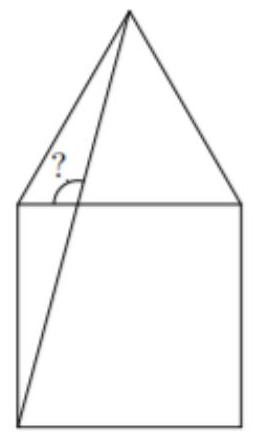
\includegraphics[max width=\textwidth, center]{2024_11_21_73a2cc92c5829e99aadag-1}\\
tylko sok?
  \item Gracza rozpoczynającego oznaczamy X, drugiego Y. Wykonują oni ruchy na przemian, przegrywa gracz, który nie może wykonać ruchu. Należy rozstrzygnąć, czy któryś z graczy ma strategię wygrywającą i wskazać zwycięzcę (jeżeli istnieje), a gra wygląda tak:
\end{enumerate}

Na okrągłym stoliku gracze kładą złotówki, przy czym nie mogą one wystawać poza stolik ani nachodzić na siebie oraz nie wolno przesuwać leżących już monet.

\section*{KLASY PO GIMNAZJUM}
\begin{enumerate}
  \item Udowodnić, że dla dowolnych liczb nieujemnych \(a, b, c\) zachodzi nierówność
\end{enumerate}

\[
\sqrt[3]{a^{2} b}+\sqrt[3]{b^{2} c}+\sqrt[3]{c^{2} a} \leq a+b+c
\]

\begin{enumerate}
  \setcounter{enumi}{1}
  \item W trapezie poprowadzono odcinek równoległy do podstaw i dzielący go na dwa trapezy o równych polach. Policz długość tego odcinka, jeżeli podstawy mają długość \(a\) i \(b\).
  \item Sfera wpisana w czworościan ABCD jest styczna do ścian ABC i ABD odpowiednio w punktach K i L. Udowodnij, że jeśli punkty K i L są środkami okręgów opisanych na trójkątach ABC i ABD to \(\Varangle A C B=\Varangle A D B\).
\end{enumerate}

\end{document}